%implementing document formatting:
%page setup (page size, text size, page layout, chapters start on a new page).
%memoir is a form of book class that supports any kind of document.
\documentclass[fleqn,a4paper,12pt,twoside,openany]{memoir}

\usepackage{titlesec}
\usepackage{anysize}
\usepackage{enumitem}
\usepackage{graphicx}


\usepackage{pifont} % extra symbols like (v.. approved)...
\usepackage[hyphens]{url}
\usepackage{array}
\usepackage{multirow}

%\titleformat{\chapter}[display]
%{\normalfont\huge\bfseries}{\chaptertitlename\ \thechapter}{20pt}{\Huge}

% this alters "before" spacing (the second length argument) to 0

\titlespacing*{\chapter}{0pt}{-50pt}{10pt}


%setting the header and footer in that order:
\setheadfoot{28pt}{28pt} %if any problems are encountered, try changing the latter 28pt with 1cm.

%general package syntax: \usepackage[options]{package}

%setting language:
\RequirePackage[danish, english]{babel}

%this package makes it possible to treat any element as a float,
%figures and tables are by default treated as floats.
%read http://en.wikibooks.org/wiki/LaTeX/Floats,_Figures_and_Captions to specify your float.
\usepackage{float}
\usepackage{wrapfig}
\usepackage{placeins}
\usepackage{siunitx}


%this package makes it possible to make theorems and examples:
\usepackage{amsthm}
%setting the style of examples (parameters: plain, definition, remark):
%(definition is usually used for examples)
\theoremstyle{definition}
%the frist parameter is the syntax used in the document, the second is that which is printed in LaTex.
\newtheorem{example}{Example}

%making it possible to use æ, ø and å:
\usepackage[utf8]{inputenc}
%helps with word division when using æ, ø and å, and makes it ps-font rather than bmp:
\usepackage[T1]{fontenc}

%package for implementation of graphic files:
\usepackage{graphicx}

%package for captions
\usepackage[nooneline]{caption}
\usepackage{subcaption}

%%package for implementation of math:
\usepackage{amsmath, amsfonts, amssymb, float, mathtools}

%allowing use of color:
\usepackage[usenames,dvipsnames]{color}
%allowing use of more colors also in tables (see: http://en.wikibooks.org/wiki/LaTeX/Colors):
\usepackage[usenames,dvipsnames,svgnames,table]{xcolor}
\usepackage{colortbl} %Colors for tabulars
\definecolor{pwdrblue}{RGB}{140,140,140} %Color changed back!
\definecolor{darkgrey}{RGB}{180,180,180}
\definecolor{lightgrey}{RGB}{241,241,241}
\definecolor{aaublue}{RGB}{53,46,102}
\definecolor{aausub}{RGB}{154,167,180}
\definecolor{MidnightBlue}{RGB}{25, 25, 112}
\definecolor{NavyBlue}{RGB}{0, 0, 128}
\definecolor{darkgray}{gray}{0.35}
\definecolor{AleeRed}{rgb}{0.5,0,0}
\definecolor{mygreen}{rgb}{0,0.6,0}
\definecolor{mygray}{rgb}{0.5,0.5,0.5}
\definecolor{mymauve}{rgb}{0.58,0,0.82}
\definecolor{UCNHeader}{RGB}{233,131,0}
%hyperlinks in the tabel of contents - comment this out before the report is printed.
\usepackage{hyperref}
\hypersetup{
	bookmarks = true,  % Show 'bookmark'-frame in pdf.
	colorlinks = false, % True = colored links, False = framed links.
	citecolor = blue,  % Link color for references.
	linkcolor = blue,  % Link color in table of contents.
	urlcolor = blue,   % Link color for extern URLs.
}

%makes it possible to refer to the name of a chapter rather than just the number.
\usepackage{nameref}
\usepackage[american,cuteinductors,smartlabels]{circuitikz}
\usepackage{tikz}
\usetikzlibrary{shapes,arrows,positioning,calc}
\usetikzlibrary{calc}
\usetikzlibrary{patterns}

%package for writing program code in latex
\usepackage{listings}

\lstset{  
  backgroundcolor=\color{lightgrey},
  %escapeinside={\%*~}{*)},
  basicstyle=\small,               
  breaklines=true,                                   
  comment=[l]{//},
  commentstyle=\color{mygreen},             
  extendedchars=false,              
  frame=none,	                                   
  keywordstyle=\color{blue},
  keywordstyle=[2]\color{red},        
  language=C,                            
  numbers=left,                   
  numbersep=5pt,                   
  numberstyle=\scriptsize,                                                                          
  stringstyle=\color{mymauve},     
  tabsize=2,	             
  morekeywords=[2]{AD1PCFG,AD1CON1, AD1CSSL, AD1CON3, AD1CON2, AD1CON1SET, AD1CHS, AD1CON1CLR, AD1CHSbits, ADC1BUF0, CH0SA},   
morekeywords={DelayUs},  
 % keywordstyle=[3]\color{blue},
  identifierstyle=\ttfamily,
  %backgroundcolor=\color{white},
}

%setting references (using numbers) and supporting i.a. Chicargo-style:

\usepackage{url}

\usepackage[backend=bibtex]{biblatex}
\bibliography{bibliography/bibliography.bib}

\usepackage{verbatim} %enables /begin(comment) and /end{comment} for larger sections

%this package makes it possible include pdf pages in fx appendix;
%using  following syntax: \includepdf[pages={1}]{myfile.pdf}
\usepackage{pdfpages}

\usepackage{pbox} % used for newline in tabular

%%%MARGINER%%%
\setlrmarginsandblock{3.5cm}{2.5cm}{*}	% \setlrmarginsandblock{inner margin}{outer margin}{ratio}
\setulmarginsandblock{2.5cm}{3.0cm}{*}	% \setulmarginsandblock{top}{bottom}{ratio}
\checkandfixthelayout 			            % fixes stuff..

%Enables the use FiXme refferences. Syntax: \fixme{...}
%With "final" in stead of "draft" an error will ocure for every FiXme
%under compilation.
%\usepackage[footnote,draft,english,silent,nomargin]{fixme}

%Centering captions in tables
%\centering
%\captionsetup{justification=centering}
%\caption{bla bla bla}
\usepackage{caption}
\usepackage{pgfplotstable}
\usepackage{pgfplots}

\pgfplotsset{width=15cm,height=7cm}
\usepackage{filecontents}
\usepackage{epstopdf}
\usepackage{nomencl}
\renewcommand{\nomname}{Glossary}
\renewcommand*{\pagedeclaration}[1]{\unskip\dotfill\hyperpage{#1}}
\makenomenclature
\usepackage{makeidx}
\makeindex

%implementing macros:
%%Figure references:
\newcommand{\figref}[1]{\textbf{figur \ref{#1}}}

%Figure references after full stop/period:
\newcommand{\Figref}[1]{\textbf{Figur \ref{#1}}}

%Table references:
\newcommand{\tableref}[1]{\textbf{tabel \ref{#1}}}

%%%CHAPTERLAYOUT%%%
%Downloaded chapter-setup:
\newif\ifchapternonum
\makechapterstyle{jenor}{
	\setlength{\beforechapskip}{-2cm}	% Adjust space between page top and chapter title.
	\setlength{\afterchapskip}{1.5cm}	% Adjust spave between chapter title and text.
  	\renewcommand\printchaptername{}
  	\renewcommand\printchapternum{}
  	\renewcommand\printchapternonum{\chapternonumtrue}
  	\renewcommand\chaptitlefont{\fontfamily{pbk}\fontseries{db}\fontshape{n}\fontsize{25}{35}\selectfont\raggedleft}
  	\renewcommand\chapnumfont{\fontfamily{pbk}\fontseries{m}\fontshape{n}\fontsize{1in}{0in}\selectfont\color{UCNHeader}}
  	\renewcommand\printchaptertitle[1]{%
    \noindent
    \ifchapternonum
    \begin{tabularx}{\textwidth}{X}
    {\let\\\newline\chaptitlefont ##1\par} 
    \end{tabularx}
    \par\vskip-2.5mm\hrule
    \else
    \begin{tabularx}{\textwidth}{Xl}
    {\parbox[b]{\linewidth}{\chaptitlefont ##1}} & \raisebox{-15pt}{\chapnumfont \thechapter}
    \end{tabularx}
    \par\vskip2mm\hrule
    \fi
  }
}
%setting chapter style:
\chapterstyle{jenor}

%depth of numbered headlines (part/chapter/section/subsection):
\setsecnumdepth{subsection}
\maxsecnumdepth{subsection}
%depth of the table of contents:
\settocdepth{section}
\parindent=0pt 

% Makes sure LaTeX does not stretch the text at page break:
\raggedbottom

\newcommand{\img}[4]{
    \begin{figure}[!ht]
    	\centering
    		\includegraphics[width=#4\textwidth]{#1}
    	\caption{\text{#2}}
    	\label{#3}
    \end{figure}
}

\newcommand{\tableimg}[3]{
    \begin{figure}[!ht]
    	\centering
    		\includegraphics[width=#3\textwidth]{#1}
    	\label{#2}
    \end{figure}
}

\newcommand{\wrapimg}[8]{
	\begin{wrapfigure}[10]{#5}{0.4\textwidth} \hspace{0pt}
	\vspace{#6}
  		\begin{center}
   			 \includegraphics[width=#4\textwidth]{#1}
  		\end{center}
  		\vspace{#7}
 		\caption{\textbf{#2}}
 	 	\label{#3}
 	 	\vspace{#8}
	\end{wrapfigure}
}

\newcommand{\sidebyimg}[4]{
	\begin{figure}[H]
		\center
		\begin{subfigure}[b]{0.48\textwidth}
			\includegraphics[width=\textwidth]{#1}
			\caption{#2}
		\end{subfigure}
		\quad
		\begin{subfigure}[b]{0.48\textwidth}
			\includegraphics[width=\textwidth]{#3}
			\caption{#4}
		\end{subfigure}
	\end{figure}
}

\newcommand{\sidebyimglabel}[8]{
	\begin{figure}[H]
		\center
		\begin{subfigure}[b]{0.48\textwidth}
			\includegraphics[width=\textwidth]{#1}
			\caption{#2}
			\label{#3}
		\end{subfigure}
		\quad
		\begin{subfigure}[b]{0.48\textwidth}
			\includegraphics[width=\textwidth]{#4}
			\caption{#5}
			\label{#6}
		\end{subfigure}
		\caption{#7}
		\label{#8}
	\end{figure}
}

\newcommand{\threesidebyimg}[9]{
	\begin{figure}[!htb]
		\minipage{0.32\textwidth}
  			\includegraphics[width=\linewidth]{#1}
  			\caption{\textbf{#2}}\label{fig:#3}
		\endminipage\hfill
		\minipage{0.32\textwidth}
  			\includegraphics[width=\linewidth]{#4}
  			\caption{\textbf{#5}}\label{fig:#6}
		\endminipage\hfill
		\minipage{0.32\textwidth}
  			\includegraphics[width=\linewidth]{#7}
  			\caption{\textbf{#8}}\label{fig:#9}
		\endminipage\hfill
	\threesidebyimgcontinued
}

\newcommand{\threesidebyimgcontinued}[1]{
	\caption{\textbf{#1}}
	\end{figure}
}

\newcommand{\blueheader}[1]{
	\cellcolor{aaublue}\textbf{\color{white}#1}
}
\begin{document}
\nomenclature{PWM}{Pulse-width Modulation}
\nomenclature{IDE}{Integrated Development Environment}
\nomenclature{MCU}{Microcontroller Unit}
\nomenclature{UART}{Universal Asynchronous Receiver/Transmitter}
\nomenclature{DC}{Direct Current}
\nomenclature{PNP}{Positive-Negative-Positive}
\nomenclature{NPN}{Negative-Positive-Negative}
\nomenclature{CPLD}{Complex Programmable Logic Devies}
\nomenclature{RTOS}{Real-Time Operating System} 
\nomenclature{MOSFET}{Metal-Oxide-Semiconductor-Field-Effect Transistor}
\renewcommand\chaptername{Chapter}
\renewcommand\contentsname{Table of Contents}
\renewcommand\figurename{Figure}
\renewcommand\tablename{Table} 

%implementing front page:
\clearpage
\thispagestyle{empty}

\begin{figure}[H]
	\raggedleft
		
\includegraphics[width=0.3\textwidth]{figures/logo-ucn.png}
\end{figure}
\vspace*{\fill} 
\begin{center}
\begin{Huge}
Fall Semester 2016\\
\vspace{5 mm}
\textbf{Autonomous Object Avoidance Robot}\\
\vspace{3 mm}
Group 2\\
\vspace{3 mm}
3. Semester IT-Technology
\end{Huge}
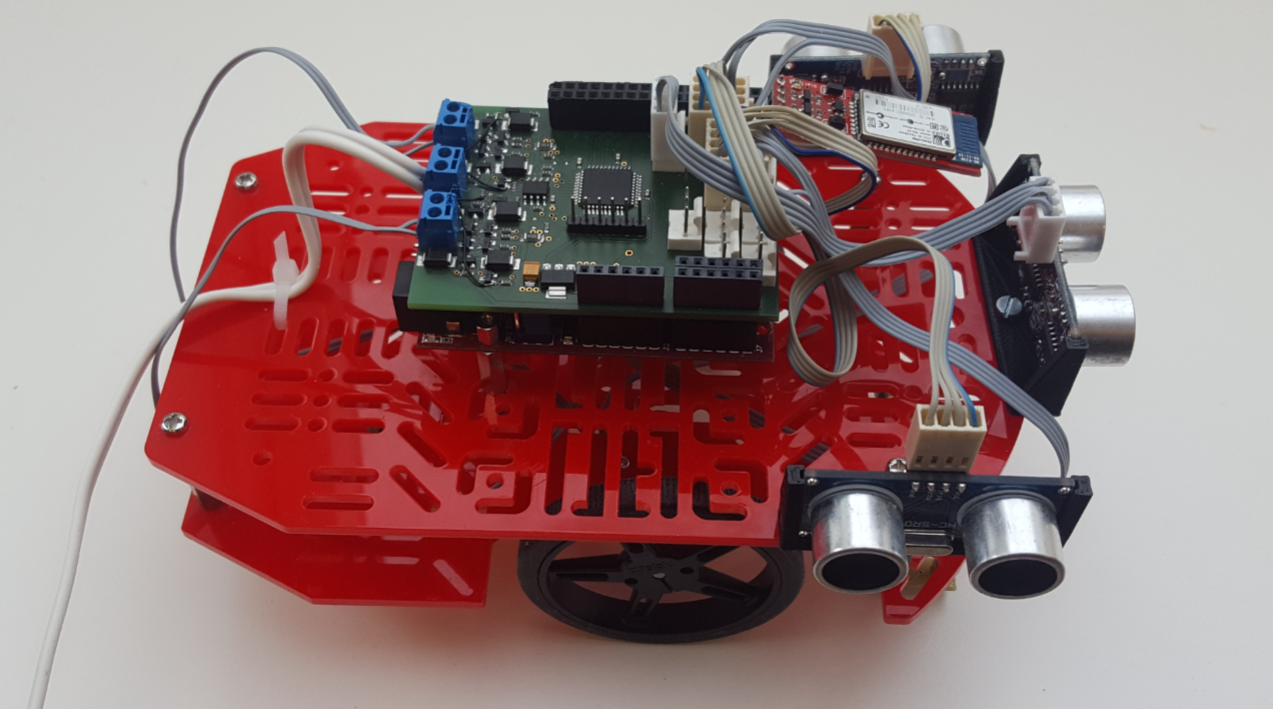
\includegraphics[width=0.7\textwidth]{figures/frontPageBot.png}
\end{center}
\vspace*{\fill}
\begin{center}
Group members:
 Benjamin Nielsen - Henrik Jensen - Martin Nonboe - Nikolaj Bilgrau
\end{center}
\begin{center}
Supervisors:Ib Helmer - Jesper Kristensen - Steffen Vutborg
\end{center}
\begin{center}
\line(1,0){400}
\end{center}
%clears one or two pages to make the document start on right hand side:
\cleardoublepage

%numbers the pages with Roman numeral - starts from "i":
\frontmatter

%implementing title sheet:
% Dette er LaTeX-versionen af titelbladet for tek-nat-basis-rapporter 2004 efterår
% Filen kræver:
% Universitetets logo:  aau-logo.png (for LaTeX) eller aau-logo.ps (for LaTeX)
% Synopsis: En fil ved navn synopsis.tex

% Udarbejdet af: Hans Håttel (hans@cs.auc.dk) 21. maj 2003
% Rettet af Morten Christophersen (mortench@tnb.aau.dk) 30. nov 2004(ændret til nyt design 2004 efterår)

%\documentclass[11pt]{article}
%\ifx\pdfoutput\undefined 
%\usepackage[dvips]{graphicx}
%\else
%\usepackage[pdftex]{graphicx} 
%\usepackage{type1cm} \fi
%    \usepackage[ansinew]{inputenc}
%    \usepackage{a4}

%\begin{document} 
\thispagestyle{empty}
%\begin{titlepage}
\begin{nopagebreak}
{\samepage 

\begin{tabular}{r}
\parbox{\textwidth}{  \raisebox{11mm}{
\includegraphics[height=1.5cm]{figures/logo-ucn.png}}
\hfill \hspace{2cm} \parbox{8cm}{\begin{tabular}{l} %4.90
{\small \textbf{\textcolor{MidnightBlue}{IT-technology}}}\\ 
{\small \textcolor{NavyBlue}{Sofiendalsvej 60}} \\
{\small \textcolor{NavyBlue}{9200 Aalborg SW}} \\
{\small \textcolor{NavyBlue}{\emph{http://www.ucn.dk/}}}
\end{tabular}}}
\end{tabular}

\begin{tabular}{cc}
\parbox{7cm}{
\begin{description}

\item { Title:} 

Autonomous Object Avoidance Robot

\end{description}

\parbox{8cm}{

\begin{description}
\item { Project Period:}\\
   3. Semester | Fall semester 2016\\
  \hspace{4cm}
\item { Projectgroup:}\\
  Group 2 
  \hspace{4cm}
\item { Group participants:}\\
Benjamin Nielsen\\
Henrik Jensen\\
Martin Nonboe\\
Nikolaj Bilgrau\\
\hspace{2cm}
\item { Supervisors:}\\
Jesper Kristensen\\
Steffen Vutborg\\
Ib Helmer Nielsen
  
\end{description}
}
\begin{description}
\item { Pages: } \fixme{fix til sidst}
\item { Appendices: } 
\item { Completed:} 
\end{description}
\vfill } &
\parbox{7cm}{
  \vspace{.15cm}
  \hfill 
  \begin{tabular}{l}
   \end{tabular}}
\end{tabular}} \vspace{1.3cm}
\centering
\\
\end{nopagebreak}
%\end{titlepage}
%\end{document}
\chapter*{Preamble}


%Læsevejledning:\\
%Kommer senere i projektforløbet.
%\\\\

TBD fyld mere på? 
This project was written by group 2, for the 3rd semester on the IT-electronics education at university college Nordjylland, Sofiendalsvej 60. The project goal is to make an autonomous robot that can navigate a course utilizing object avoidance and localization.
%
\phantom{Luft}\vspace{3cm}
\begin{table}[H]
	\centering
		\begin{tabular}{c c c}
			\underline{\phantom{JAERJAERJAERJAERGO}} & \phantom{cookies} & \underline{\phantom{JAERJAERJAERJAERGO}} \\
			Benjamin Nielsen			& \phantom{cookies} & Henrik Jensen		\\
			&&\\
			&&\\
			\underline{\phantom{JAERJAERJAERJAERGO}} & \phantom{cookies} & \underline{\phantom{JAERJAERJAERJAERGO}} \\
			Martin Nonboe			& \phantom{cookies} & Nikolaj Bilgrau		\\
			&&\\
						
		\end{tabular}
\end{table}

\cleardoublepage

%the '*' allows the tableofcontents be excepted from the actual table of contents.
\tableofcontents*
\newpage
\printnomenclature
\renewcommand*\listfigurename{List of Figures}
\renewcommand*\listtablename{List of Tables}

%numbers the pages with Arabic numeral - starts from 1.
\mainmatter
\chapter{Introduction}
In countries with high wages and where manual labour is expensive, the industrial production is often organized as an automated process. To make the whole industry smarter and more customizable, new automated robots and reliabilities are needed. The many new forms of robots rely on sensors to face the many different challenges.
Automation of movement and avoidance enables even robotic space exploration, as seen in the many rovers visiting the different nearby planets. \
 \\

There are different sensors in play when needing to avoid obstacles or collision. To mention a few, ultrasound, infra-red and laser sensors comes to mind, all of which are viable picks when building a robot with object avoidance.\\

In the project at hand, we will be focusing mainly on the ultrasound sensor for building an object avoiding robot. 
The objective of this project is to design and implement an automotive robot capable of autonomous object manoeuvring, specially a collision avoiding robot employing light detecting sensing and ultrasound sensing.\\

The project was handed to the group at the start of third semester and is to be handed in at the 9th of January, 2017.
\chapter{Analysis}
Indledning til afsnittet af analyse\\

\section{Problem statement}

The problem presented to the group is how to make a robot move from point A to point B, with the help of different sensors, including ultrasound and infrared, and to make use of autonomous  to avoid obstacles. \\


Problem statement \\
- Bot should be able to move from A to B.\\
- Should be able to stop at B\\
- Manoeuvre around obstacles\\
- Optimize speed of bot
- 

\section{Problem analysis}

\chapter{Requirements specification}
This section specifies the requirements. The requirements have been found through the analysis.

\cite{ucn}
\begin{enumerate}
	\item[•]The robot needs line following capabilities\\
	\item[•]The robot needs object avoidance\\
	\item[•]The robot should make use of an H-bridge\\
	\item[•]The robot should make use of Motors\\
	\item[•]The robot needs a way to implement motor control\\
	\item[•]The robot should make use of a micro-controller unit\\
	\item[•]The robot should make use of the Magician chassis\\
\end{enumerate}


\chapter{Hardware section}
%\subsection{Hardware diagram}
%Hardware Diagram
%\section{Description of the hardware structure and functionality}
In this section the different components of the hardware will be listed, described & explained.

\section{Hardware diagram}
Beskrivelse af hardware diagram


\subsection{Object avoidance sensor choices}
SR04 Ultrasound
GP2Y0A02YK0F (long) \\	
GP2Y0A41SK0F (short) \\
\\
\subsection{Line following sensor choice} 

QRE1113 - 
\section{Analog-to-digital converter}


\subsubsection{ADC diagram} 

\subsubsection{The usage of ADC}

\section{The chipKIT Uno32 board}


\section{The motor shield - PKA03}

\subsection{The H bridge}


\section{The Bluetooth tranceiver}


\input{contents/hardware/partconclusion.tex}
\chapter{Software section}
%\input{contents/software/softwarespec.tex}

Beskriv Software section

\subsection{Software diagram}

\section{Analog to digital conversion}
%\begin{lstlisting}
%\end{lstlisting}

\section{Pulse-width modulation}

\subsection {Why utilize pulse-width modulation}

Pulse-width modulation, or PWM, is a way to regulate power distribution within a system. It is a software solution that manages when a device receives power, and for how long at a time it does this. This is called a duty cycle. The robot utilizes PWM for its motors, to regulate how quickly it moves. PWM can be compared to turning a switch on and off extremely quickly - much more quickly than what will affect the performance of the motors. Effectively, this means that the robot's programming will now be able to regulate speed autonomously. 
 
\subsection {Duty cycles}

The duty cycle is used to describe how long the power is 'on' compared to 'off'. A higher duty cycle will yield more energy than a low one. The programming uses a frequency of 1000Hz, which makes it straightforward to calculate to real time, if this is needed - it also provides enough precision to make the motors responsive quickly.

\section{The interface}

\section{Part conclusion}
Software problemer og løsninger
\input{contents/software/partconclusion.tex}
\chapter{Test}
To make sure the product as a whole is working according to plan, testing must be done. First the components must be tested, this is done individually for each component to make sure there are no errors or fails when the product is built. The purpose of integration testing is to detect any inconsistencies between the software units that are integrated together. Testing is also done to watch the behavior of the product and tweak it.

\section{Unit Testing}
The individual parts of the system will be tested in the following section
\subsection{Sensor}
The following test is to make sure that the selected sensors work as intended for the project.

\subsubsection{Equipment}
\begin{enumerate}
    \item[•]Hameg HM8040-2 Triple Power Supply
	\item[•]Fluke 45 Multimeter
\end{enumerate}

\subsubsection{Setup}
Sensor is powered through the robot.
Output from sensor is measured with multimeter.

\subsubsection{Results}
\textbf{White Surface:}
Average voltage measured: 230 mV\newline
\textbf{Black Surface:}
Average voltage measured: 2,6 V\newline
This shows that the sensor clearly measures a difference between light and dark surfaces, making it ideal for this application.

\subsection{DC Motors}
The following test is to make sure that the DC motors work as intended.

\subsubsection{Equipment}
\begin{enumerate}
	\item[•]Hameg HM8040-2 Triple Power Supply
	\item[•]Fluke 45 Multimeter
\end{enumerate}

\subsubsection{Setup}
The motor is powered through the power supply.
Amount of drawn current is measured with multimeter.

\subsubsection{Results}
Both motors have been measured at 6 V and show a steady current draw of 0,11 A when running freely.


\subsection{H-Bridge}
The following test is to make sure the H-bridge works as intended.

\subsubsection{Equipment}
\begin{enumerate}
	\item[•]Hameg HM8040-2 Triple Power Supply
	\item[•]Fluke 45 Multimeter
	\item[•]Agilent MSO-X 3024A Oscilloscope.
\end{enumerate}

\subsubsection{Setup}
H-Bridge is powered by the power supply.
PWM and duty cycle is controlled by the function generator in the Oscilloscope.
Output is measured with the multimeter.
H-bridge motor direction is controlled manually.

\subsubsection{Results}
\textbf{Direction: 0}
\begin{enumerate}
	\item[•]\textbf{Duty Cycle 20\%:} 1,76 V measured.
	\item[•]\textbf{Duty Cycle 50\%:} 2,74 V measured.
	\item[•]\textbf{Duty Cycle 80\%:} 3,58 V measured.
\end{enumerate}

\textbf{Direction: 1}
\begin{enumerate}
	\item[•]\textbf{Duty Cycle 20\%:} -1,57 V measured.
	\item[•]\textbf{Duty Cycle 50\%:} -2,55 V measured.
	\item[•]\textbf{Duty Cycle 80\%:} -3,50 V measured.
\end{enumerate}

The results show that the H-Bridge unit is capaple of controlling the voltage output in both directions, with the output voltage level controlled by the PWM signal applied to the unit.

\subsection{PWM}
This test is to measure the PWM capability of the PIC32MX320F128H as well to see is the software implementation is capable of controlling the PWM module of the MCU.

\subsubsection{Equipment}
\begin{enumerate}
	\item[•]Agilent MSO-X 3024A Oscilloscope.
	\item[•]chipKIT Uno32 with PICkit 3 programmer.
\end{enumerate}

\subsubsection{Setup}
The Uno32 board is programmed to run the PWM at different frequencies and duty cycles.
Output is measured with the Oscilloscope.

\subsubsection{Results}
The test shows that the PWM module and developed software is working as intended.
\img{figures/f1000d20.png}{Output with 1000 Hz frequency and 20\% Duty Cycle}{f1000d20}{0.7}
\img{figures/f1000d50.png}{Output with 1000 Hz frequency and 50\% Duty Cycle}{f1000d50}{0.7}
\img{figures/f1000d80.png}{Output with 1000 Hz frequency and 80\% Duty Cycle}{f1000d80}{0.7}
\img{figures/f10000d50.png}{Output with 10000 Hz frequency and 50\% Duty Cycle}{f10000d50}{0.7}\newpage

\subsection{ADC}
This test is to show that the ADC module and the developed software for the module is working as intended.

\subsubsection{Equipment}
\begin{enumerate}
	\item[•]Hameg HM8040-2 Triple Power Supply.
	\item[•]chipKIT Uno32 with PICkit 3 programmer in debug mode.
\end{enumerate}

\subsubsection{Setup}
The Uno32 is powered from the PICkit 3 programmer in debug mode to read the contents of a variabel containing the output of the ADC module.
The input voltage on the ADC is supplied by the power supply.

\subsubsection{Results}
\begin{enumerate}
	\item[•] \textbf{PS:} 0,499V - \textbf{Measured:} 163 (0,526V) - \textbf{Error:} 5,3\%
	\item[•] \textbf{PS:} 1,000V - \textbf{Measured:} 331 (1,068V) - \textbf{Error:} 6,7\%
	\item[•] \textbf{PS:} 2,006V - \textbf{Measured:} 665 (2,145V) - \textbf{Error:} 6,4\%
	\item[•] \textbf{PS:} 3,299V - \textbf{Measured:} 1023 (3,300V) - \textbf{Error:} 0,03\%
\end{enumerate}
This shows that the ADC and the developed software works within the required area for the application.
\newpage
\section{Integration Testing}

\subsection{PWM motor control}
The following test is to show that the DC motors can be controlled by the H-bridge unit.

\subsubsection{Equipment}
\begin{enumerate}
	\item[•]Hameg HM8040-2 Triple Power Supply.
	\item[•]chipKIT Uno32 with PICkit 3 programmer.
\end{enumerate}

\subsubsection{Setup}
	The H-bridge module is powered from the power supply.
	The control signals is controlled by the Uno32 board.

\subsubsection{Results}
\begin{enumerate}
	\item[•]\textbf{PWM: 20\%:} Motors are not turning. Audible whine.
	\item[•]\textbf{PWM: 30\%:} Motors are not turning. Higher audible whine.
	\item[•]\textbf{PWM: 37\%:} Motors are turning slowly with assisted start.
	\item[•]\textbf{PWM: 40\%:} Motors are turning slowly.
	\item[•]\textbf{PWM: 100\%:} Motors are turning maximum speed.
\end{enumerate}
This shows that we the current setup of Motors and H-bridge unit, the variable control span is between an duty cycle of 37\% and 100\%.

\subsection{Robot to Interface communication}
This test is to show that the system is capable of transmitting current data from the robot to the interface and accurately show it to the user.

\subsubsection{Equipment}
\begin{enumerate}
	\item[•]chipKIT Uno32 with PICkit 3 programmer.
	\item[•]BlueSMIRF silver Bluetooth module.
	\item[•]PC running C\# interface.
\end{enumerate}

\subsubsection{Setup}
The robot is placed so that the sensors measures over a white and a black surface.
data is sent over bluetooth to the interface and data recorded.

\subsubsection{Results}
\sidebyimg{figures/sensorsonwhite.png}{Interface showing data sent with sensors placed over white surface}{figures/sensorsonblack.png}{Interface showing data sent with sensors placed over black surface}

\section{System Testing}
This test is to show that the system works as intended.

\subsubsection{Equipment}
\begin{enumerate}
	\item[•]chipKIT Uno32 with PICkit 3 programmer.
	\item[•]BlueSMIRF silver Bluetooth module.
	\item[•]PC running C\# interface.
\end{enumerate}

\subsubsection{Setup}
The system is tested by placing the robot in 3 different situations.
\begin{enumerate}
	\item[•]Centered on line.
	\item[•]Line at the right end of sensor array.
	\item[•]Line at the left end of sensor array.
\end{enumerate}
\newpage
\subsubsection{Results}
\img{figures/interfacestraight.png}{Only the middle sensor is detecting the line}{interfacestraight}{0.5}
\sidebyimg{figures/interfaceleftturn.png}{Sensor on the left detects line, initiate left turn}{figures/interfacerightturn.png}{Sensor on the right detects line, initiate right turn}
\newpage
\section{Acceptance Testing}
This test is to show that the product as a whole works on a simple test track.

\subsubsection{Equipment}
\begin{enumerate}
	\item[•]Complete robot with working control software
	\item[•]Test track
\end{enumerate}

\subsubsection{Setup}
The robot is calibrated on the test track and placed on the line. The robots behaviour is recorded and deemed acceptable or not.

\subsubsection{Results}
The robot drives acceptably on the track most of the time. Other times, it seems to overshoot on the corners. See attached videos for example tests.






\chapter{Conclusion}
TBD
Skriv en fucking Conclusion!!
\chapter{Appendices}
TBD hele den her section
\section{Group collaboration agreement}
\subsection{Contact Information}
\begin{table}[h!]
\centering
\caption{Contacts}
\label{Contact info}
\begin{tabular}{|l|l|l|}
\hline
Benjamin Nielsen & Tlf: 30427645 & @: yipiyuk5@gmail.com       \\ \hline
Henrik Jensen    & Tlf: 28568934 & @: henrik\_kort@hotmail.com \\ \hline
Martin Nonboe    & Tlf: 23827566 & @: nonsens\_4@hotmail.com   \\ \hline
Nikolaj Bilgrau  & Tlf: 29802715 & @: nikolajbilgrau@gmail.com \\ \hline
\end{tabular}
\end{table}

\subsection{Workflow}


\subsection{Deadline}
\subsubsection{Hardware}
The hardware part of the project was supposed to be ready before the 22th 
\subsubsection{Software}

\subsection{Milestones and goals}
Gerne en kalender der viser dage arbejdet!
\chapter{List of references}

%\url{}\\


\newpage
\listoffigures
\addtocontents{lof}{~\hfill\textbf{Page}\par}
\newpage
\listoftables
\addtocontents{lot}{~\hfill\textbf{Page}\par}
\newpage
\chapter{Hardware appendix}
\section{Hardware Schematics}

\subsection{H-bridge 1}
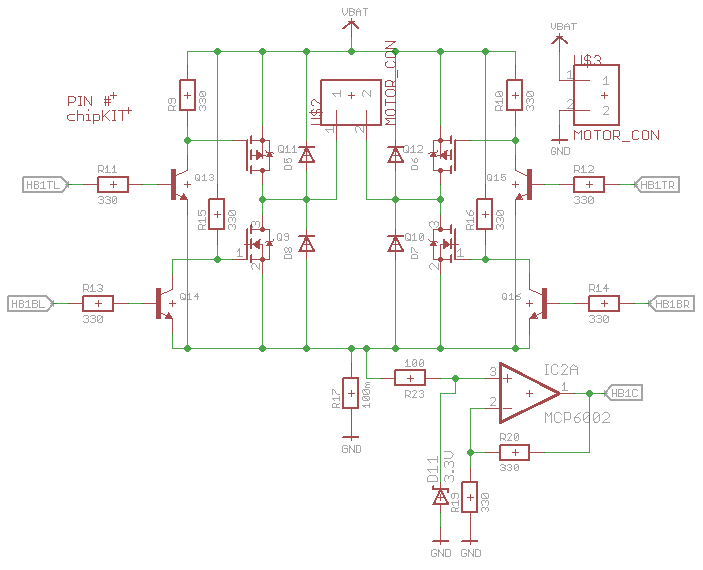
\includegraphics[width=0.7\textwidth]{figures/HB1.PNG}
\subsection{H-bridge 2}
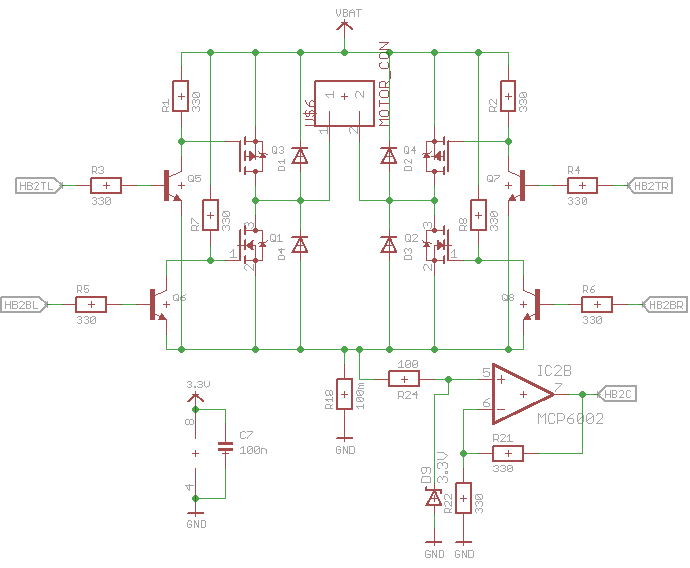
\includegraphics[width=0.7\textwidth]{figures/HB2.PNG}

\subsection{CPLD}

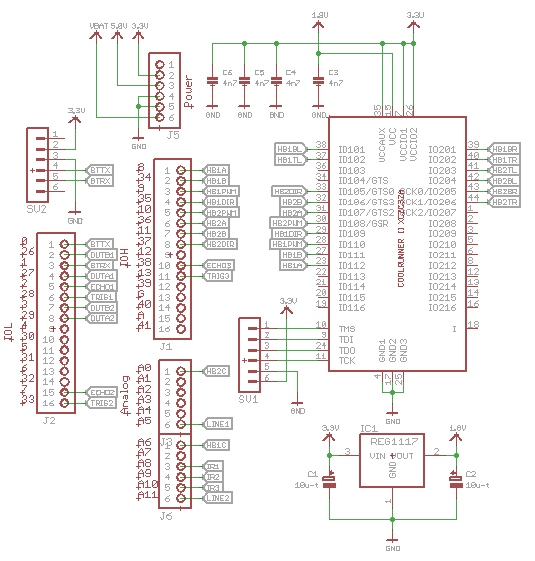
\includegraphics[width=0.7\textwidth]{figures/CPLD.PNG}

\subsection{Power}

\includegraphics[width=0.7\textwidth]{figures/Power.PNG}

\subsection{Board schematics}
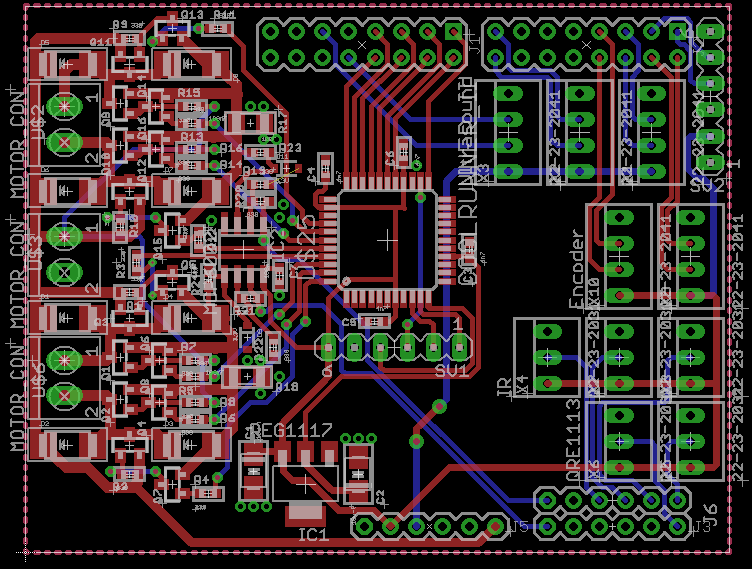
\includegraphics[width=0.7\textwidth]{figures/BoardSche.PNG}
\chapter{Software appendix}
\section{Hardware errors}
HB1A = 1 \\
HB1B = 0\\

HB1DIR = HIGH\\
HB1PWM = HIGH\\
HB1A = HIGH\\
HB1B = LOW\\

HB1TL = HIGH\\
HB1BL = HIGH - Q14 - R13 (PROBLEM) = 0\\
HB1BR =LOW\\
HB1TR = LOW\\

HB2TL = LOW\\
HB2BL = HIGH\\
HB2BR = HIGH\\
HB2TR = LOW\\

HB1A = 0\\
HB1B = 1\\

HB1DIR = HIGH\\
HB1PWM = HIGH\\
HB1B = HIGH\\
HB1A = LOW\\

HB1TL = LOW\\
HB1BL = LOW\\
HB1BR = HIGH \\
HB1TR = HIGH\\

HB2TL = LOW\\
HB2BL = HIGH\\
HB2BR = HIGH\\
HB2TR = LOW\\
\section{C code}
main.c:

%\begin{lstlisting}
%\end{lstlisting}
\newpage
ADC.c:
%\begin{lstlisting}
%\end{lstlisting}
\newpage
\section{C\# code - interface}
\lstset{language=[Sharp]C}
\begin{lstlisting}

\end{lstlisting}
\printbibliography
\listoffixmes
\end{document}